\begin{center} 
\emph{``Education is that whole system of human training within and without the school house walls, which molds and develops men.'' -- W. E. B. Du Bois}
\end{center}

\section{Linear Systems}\label{sec:linearsystems}
%\setcounter{Thm}{8}
\setlength{\columnsep}{40pt}
%\renewcommand{\arraystretch}{2.}
\emph{In this section, we introduce the study of linear systems motivated by geometry. Thus, all numbers in this section will be real numbers. We introduce the notion of a system of linear equations and the nature of their solution sets. We discuss when a linear system is consistent/inconsistent, independent/dependent, underdetermined/overdetermined, and homogeneous/nonhomogeneous. We discuss the difference between free and dependent variables in a linear system.}

\begin{Def}\label{def:linearsystem} A \textbf{system of linear equations}\index{linear system} (or a \textbf{linear system}) is a set of equations with common variables of the following form:
\[a_1x_1+a_2x_2+\ldots+a_nx_n = b,\] where $b$ and the \textbf{coefficients} $a_1, \ldots, a_n$ are fixed numbers.\\

 A \textbf{solution} to a system is an assignment to each variable such that each equation is satisfied. The \textbf{solution set} is the set of all solutions to a system of equations. Two systems of equations are \textbf{equivalent} if they have the same solution set.
\end{Def}

A linear equation of two real variables (typically $x, y$ or $x_1, x_2$) geometrically forms a \emph{line} in the plane. Likewise, a linear equation of three real variables (typically $x, y, z$ or $x_1, x_2, x_3$) geometrically forms a \emph{plane} in 3-space. Although much harder to visualize, a linear equation in four variables (typically $x, y, z, w$ or $x, y, z, t$ or $x_1, x_2, x_3, x_4$) geometrically forms a \emph{hyperplane} in 4-space. Higher dimensional analogues likewise exist. As such, emphasis in this section will be placed on linear systems with two or three real variables. \\

\begin{multicols}{2}
\begin{Exam}\label{exam:1.1firstgeom} Test that $(3,1)$ is a solution to the system \[\begin{linear} &x\ &+\ &5&y\ &=\ &8& \\ 2&x\ &-\ &&y\ &=\ &5&.  \end{linear}\]   

Notice that $3+ 5(1) = 3+5 = 8$ and $2(3) - 1 = 6 -1 = 5$. Thus, $(3,1)$ is a solution to the above system.\\

Geometrically, the solution to the previous system is an intersection between two lines, as depicted to the right. \vspace{-0.2 in}
\begin{center}
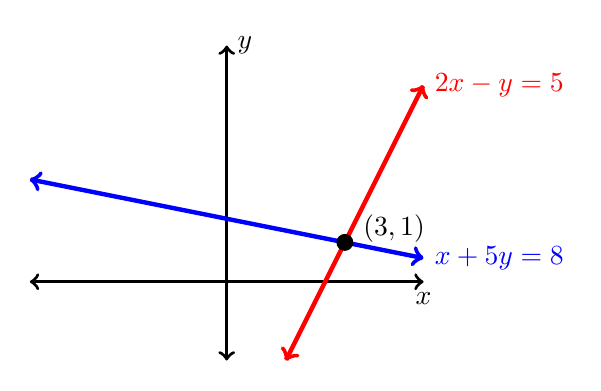
\begin{tikzpicture}[scale= .5]
\draw[<->, very thick] (-5,0) -- (5,0)node[below] {$x$};
\draw[<->, very thick] (0,-2) -- (0,6) node[right] {$y$};

\draw[red, ultra thick, domain = 1.5:5, samples = 400, <->] plot (\x, {2*\x-5}) node[right] {$2x-y=5$};
\draw[blue, ultra thick, domain = -5:5, samples = 400, <->] plot (\x, {-\x/5+8/5}) node[right] {$x+5y=8$};

\draw (4.25,1.35) node {$(3,1)$};
\draw[fill] (3,1) circle (.2);
\end{tikzpicture}
\end{center}
\end{Exam}
\end{multicols}\vs

\begin{Exam} \label{exam:1.1firstthree} Consider the linear system with three variables and three equations: \[\begin{linear} x\ &+\ &2y\ &+\ &3z\ &=\ &20\\ -2x\ &+\ &y\ &&\ &=\ &-1\\ -3x\ &-\ &6y\ &+\ &5z\ &=\ &-4. \end{linear}\] %Mariah Clayson

We can check that $(2,3,4)$ is a solution of this system. Note that $(2) + 2(3) + 3(4) = 2+8+12=20\ \checkmark$, $-2(2) + (3)  = -4+3=-1\ \checkmark$, and $-3(2) - 6(3) + 5(4) = -6-18+20 = -4\ \checkmark$, which shows that $(2,3,4)$ is in fact a solution of the system. Try as one might, another solution to this system CANNOT be found, that is, $(2,3,4)$ is the unique solution to this system of equations.
\end{Exam}

\begin{Exam}\label{exam:1.1dependent} Consider the linear system with three variables and three equations: \[\begin{linear} 2x\ &-\ &y\ &+\ &z\ &=\ &11\\ x\ &+\ &3y\ &-\ &10z\ &=\ &2\\ -3x\ &+\ &2y\ &-\ &3z\ &=\ &-17&. \end{linear}\] %Daven Triplett

It is simple to check that $(5,-1,0)$ is a solution to this system. Likewise, we can also show that $(6,2,1)$ is a solution to this same system. Thus, it is possible to have multiple solutions to a linear solutions.
\end{Exam}\vs

Because of \examref{exam:1.1dependent}, it is worth investigating how many solutions a linear system may have. The beginning of our investigation is the following definitions.\\


\begin{Def}\label{def:consistent} A system of equations is \textbf{consistent} if it has a solution. Otherwise, we call the system \textbf{inconsistent}.\\

If a consistent linear system has a unique solution, we call this the \textbf{independent case}.\label{def:uniquesoln} If a consistent linear system has multiple solutions, we call this the \textbf{dependent case}.\end{Def}\vs

Like we did in \examref{exam:1.1firstgeom}, we will investigate linear systems with two variables and their corresponding geometry.\\

\begin{Exam} Solve each system of equations. 
\begin{enumerate}
\begin{multicols}{2}
\item $\begin{linear} 
5x\ &+\ &2y\ &=\ &32\\
3x\ &+\ &6y\ &=\ &48 
\end{linear}$\\

After graphing the two lines, as depicted to the right, we see that the two lines intersect at a unique point. This point of intersection, \fbox{$(4,6)$}, means the system has a unique solution. Therefore, the system is consistent and independent.\\

\begin{center}
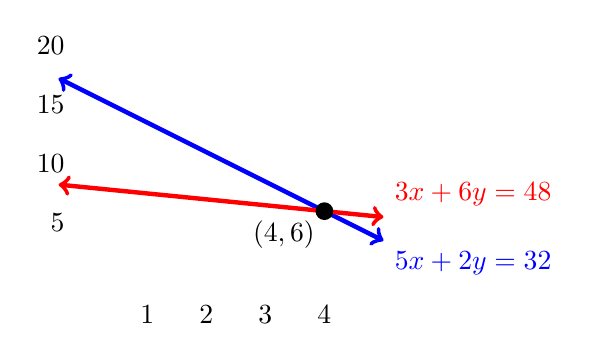
\begin{tikzpicture}[scale = 0.75]
\gridlines{-0.5}{5}{-0.5}{5};
\node[below, yshift= -5] at (1,0) {$1$};
\node[below, yshift= -5] at (2,0) {$2$};
\node[below, yshift= -5] at (3,0) {$3$};
\node[below, yshift= -5] at (4,0) {$4$};
\node[left, xshift= -5] at (0,1) {$5$};
\node[left, xshift= -5] at (0,2) {$10$};
\node[left, xshift= -5] at (0,3) {$15$};
\node[left, xshift= -5] at (0,4) {$20$};

\draw[ultra thick, blue, <->] plot[domain = -0.5:5] ({\x}, {-1/2*\x + 16/5}) node[below right] {$5x+2y=32$};
\draw[ultra thick, red, <->] plot[domain = -0.5:5] ({\x}, {-1/10*\x + 8/5}) node[above right] {$3x+6y=48$};
\fill (4, 6/5) circle (0.15) node[below left] {$(4,6)$};
\end{tikzpicture}
\end{center}
\end{multicols}

\begin{multicols}{2}
\item $\begin{linear} 
&&y\ &=\ &-x\ &+\ &5\\
2x\ &+\ &2y\ &=\ &3 
\end{linear}$\\

After graphing the two lines, as depicted to the right, we see that the two lines are parallel. Thus, they do NOT ever intersect. Therefore, the system is \fbox{inconsisitent}, that is, there is no solution to the linear system.\vfill

\begin{center}
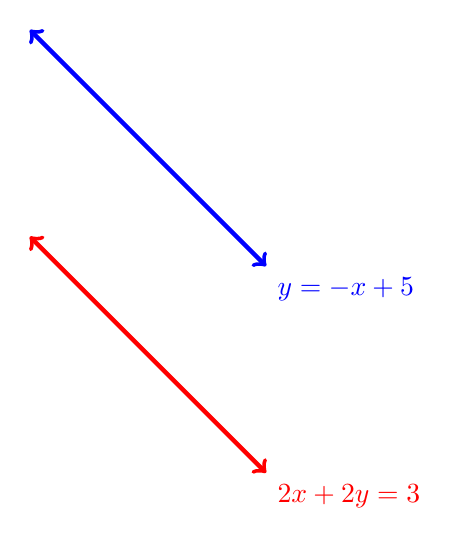
\begin{tikzpicture}[scale = 0.75]
\gridlines{-2}{2}{-1}{7};

\draw[ultra thick, blue, <->] plot[domain = -2:2] ({\x}, {-\x+5}) node[below right] {$y=-x+5$};
\draw[ultra thick, red, <->] plot[domain = -2:2] ({\x}, {-\x+1.5}) node[below right] {$2x+2y=3$};
\end{tikzpicture}
\end{center}
\end{multicols}
\pagebreak
\begin{multicols}{2}
\item $\begin{linear} 
&&x\ &=\ &\dfrac{2}{3}y\ &+\ &3\\
3x\ &-\ &3y\ &=\ &9 
\end{linear}$\\

After graphing the two lines, as depicted to the right, we see that the two lines are the same line. Thus, every point on one line is also a point on the other line. Therefore, the system is dependent, that is, there are infinitely many solutions to the linear system. In particular, the system is consistent.\vfill

\begin{center}
\begin{tikzpicture}[scale = 0.75]
\gridlines{-1}{6}{-3}{3};

\draw[ultra thick, blue, <->] plot[domain = -3:3] ({2/3*\x+3}, {\x}) node[below right] {$x=\dfrac{2}{3}y+3$};
\draw[ultra thick, dashed, red, <->] plot[domain = -3:3] ({2/3*\x+3}, {\x}) node[left, xshift=-3] {$3x-3y=9$};
\end{tikzpicture}\hfill$\qedhere$
\end{center}
\end{multicols}

\end{enumerate}
\end{Exam}

In general, any two lines in the real plane intersect at  0, 1, or infinitely many points (this last case occurs if the lines overlap). This holds also for higher dimensional systems of linear equations, that is, for any system of linear real equations the number of solutions is 0, 1, or $\infty$ and the solution set of a linear system will fall under one of these three types.\\

 These three possibilities are also the case for intersections of planes in 3-dimensional space. The \hyperref[def:consistent]{\emph{independent, consistent}} case occurs when all planes in the system intersect at a unique point. This was the case for \examref{exam:1.1firstthree}. Visually, this can be seen as three planes intersecting at a unique point, such as the three planes involved in \examref{exam:1.1firstthree}, illustrated below:
\begin{center} 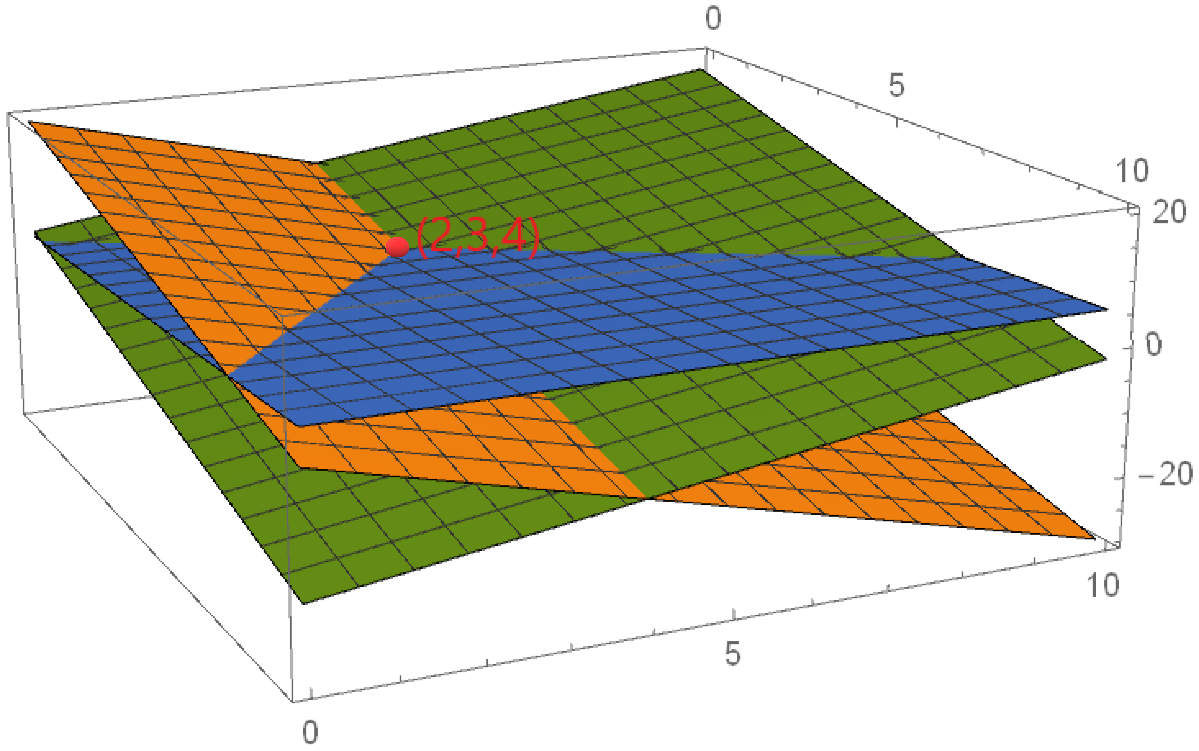
\includegraphics[scale=.25]{Chapter1/images/1-1firstthree.png} \end{center}%Mariah Clayson
The \hyperref[def:consistent]{\emph{inconsistent}} case occurs when not all the planes simultaneously intersect at a common point, perhaps because some subset of planes are parallel with one another. Finally, the \hyperref[def:consistent]{\emph{dependent, consistent}} case occurs when the collection of planes overlay at more than one point, e.g. three planes in 3-space intersect along a common line, as illustrated below: 
\begin{center} 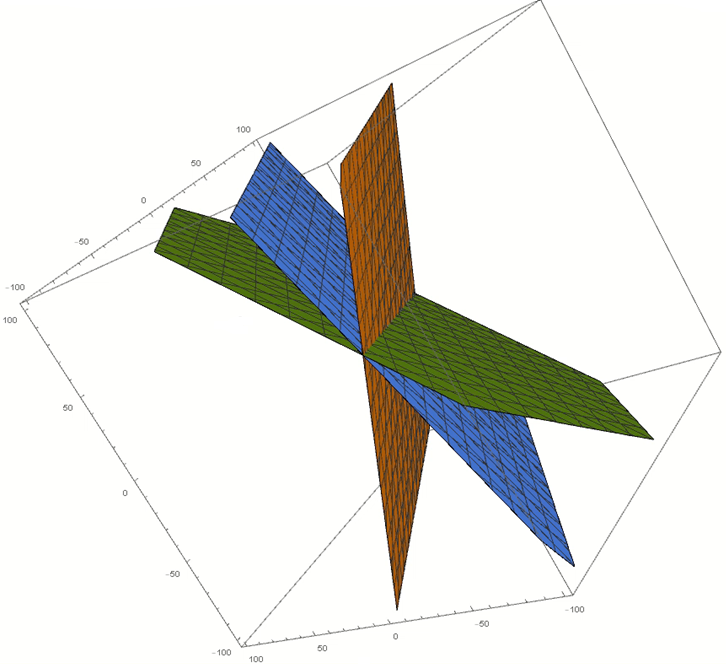
\includegraphics[scale=.35]{Chapter1/images/1-1secondthree.png} \end{center}%Greg Walsh 
This was the case for \examref{exam:1.1dependent}. In fact, any point of the form 
\setcounter{equation}{\value{Thm}} \begin{equation}\label{exam:generalform} (z+5, 3z-1,z), \end{equation} \stepcounter{Thm}
 where the variable $z$ can be freely assigned to any real number, is a solution to this linear system. This is called the \textbf{general solution} to the system. In this example, $z$ is a \mbox{\label{def:freevar}\textbf{free variable},} that is, a variable which can be assigned any value. The other two variables, $x$ and $y$, are called \textbf{dependent variables}, because their assignment is dependent upon the assignments of the free variables corresponding to some linear relationship. Thus, the linear system in \examref{exam:1.1dependent} has one free variable and two dependent variables. The two solutions listed in \examref{exam:1.1dependent} arose exactly from setting $z=0$ and $z=1$, respectively. In general, the dependent case occurs exactly when the linear system has at least one free variable. \\

The following properties will be proven in the homework.\\

\begin{Prop} \label{prop:1.1determine} Suppose that a consistent linear system has $m$ equations and $n$ variables. 
\begin{enumerate}[label=(\roman*), series=!THM!]
\item  If $n > m$, then the system has at least $n-m$ free variables which implies that it has multiple solutions.\\
\item If $m > n$, then the system has at least $m-n$ many equations which could be removed without modifying the solution set.
\end{enumerate}
\end{Prop}\vs

The situation where $n >m$ is called an \textbf{underdetermined system} because there are not enough equations to guarantee a unique solution. The situation where $m >n$ is called an \textbf{overdetermined system} because there might be too many equations to guarantee consistency. 

\begin{Def}\label{def:homogeneous} A system of linear equations is called \textbf{homogeneous} if each equation is of the form:
\[a_1x_1+a_2x_2+\ldots+a_nx_n = 0.\] Otherwise, the system is called \textbf{nonhomogeneous}.\\
\end{Def}


\begin{Exam}  The below $3\times 3$ linear system is homogeneous since the right hand side of each equation is 0: %Seth Palmer
\[\begin{linear} x\ &+\ &3y\ &+\ &5z\ &=\ &0\\
2x\ &+\ &4y\ &+\ &6z\ &=\ &0\\
4x\ &+\ &2y\ & & &=\ &0
\end{linear}\]

On the other hand, the below linear system appears to be homogeneous at first, but is really non-homogeneous: %Malcolm Hanks
\[\begin{linear} x\ &+\ &3y\ &-\ &2z\ &+\ &4\ &=\ &0\\
4x\ &+\ &2y\ &+\ &3z\ &-\ &5\ &=\ &0\\
-x\ &+\ &5y\ &-\ &3z\ &-\ &2\ &=\ &0
\end{linear}\] The issue here is that the linear system is not in \emph{standard form}, that is, all the variables are located on the left-hand sides of the equations, in descending order, and the constants are all on the right-hand sides of the equations. In standard form, the system would appear as:
\[\begin{linear} x\ &+\ &3y\ &-\ &2z\ &=\ &-4\\
4x\ &+\ &2y\ &+\ &3z\ &=\ &5\\
-x\ &+\ &5y\ &-\ &3z\ &=\ &2&0
\end{linear}\] In standard form, it is much more clear that the above linear system is non-homogeneous.
\end{Exam}\vs

\begin{Prop}\label{prop:1.1homo} A homogeneous system of equations is always consistent. \end{Prop}

%%%%%%%%%%%%%%%%%%% Exercises %%%%%%%%%%%%%%%%%%%
\startExercises{linearsystems}

\noindent For Exercises \ref{exer:checksolutionsecondstart}--\ref{exer:checksolutionsecondstop}, determine if the point is a \hyperref[def:linearsystem]{solution to the following linear system}\\  $\begin{linear} x\ &+\ &y\ &&&=\ &7\\ 3x\ &+\ &3y\ &-\ &10z\ &=\ &-79\\ x\ &+\ &5y\ &+\ &z\ &=\ &33&.\end{linear}$  %Cameron Dix
\begin{multicols}{4}
\begin{enumerate}[series=!HW!, label=\arabic*., ref=\arabic*]
\item \label{exer:checksolutionsecondstart} $(4,3,10)$ 
\item $(0,0,0)$
\item $(3,4,10)$
\item\label{exer:checksolutionsecondstop} $(-10,3,-38)$
\end{enumerate}
\end{multicols}\vs

\noindent For Exercises \ref{exer:checksolutionfirststart}--\ref{exer:checksolutionfirststop}, determine if the point is a \hyperref[def:linearsystem]{solution to the following linear system}\\ $\begin{linear} x\ &+\ & 3y\ &-\ &2z\ &=\ &13\\ 2x\ &-\ &y\ &&&=\ &2\\ -x&+\ &6y\ &-\ &4z\ &=\ &17&.\end{linear}$   %Abby Allen
\begin{multicols}{4}
\begin{enumerate}[!HW!, label=$\spadesuit$ \arabic*., ref=\arabic*]
\item\label{exer:checksolutionfirststart} $(6,10,4)$
\item $(5,8,8)$ 
\item $(3,4,1)$
\item \label{exer:checksolutionfirststop} $(9,3,2)$
\end{enumerate}
\end{multicols}\vs


\noindent For Exercises  \ref{exer:checksolutionthirdstart}--\ref{exer:checksolutionthirdstop}, determine if the point is a \hyperref[def:linearsystem]{solution to the following linear system}\\ $\begin{linear} x\ &-\ & y\ &+\ &z\ &=\ &5\\ 3x\ &+\ &4y\ &-\ &5z\ &=\ &-2\\ -2x&-\ &4y\ &+\ &7z\ &=\ &11&.\end{linear}$   %anon
\begin{multicols}{5}
\begin{enumerate}[!HW!]
\item\label{exer:checksolutionthirdstart} $(1,2,3)$
\item $(3,2,1)$ 
\item $(5,0,6)$
\item $(3,1,3)$
\item \label{exer:checksolutionthirdstop} $(9,3,2)$
\end{enumerate}
\end{multicols}\vs

\noindent For Exercises \ref{exer:dependentsystemstart}--\ref{exer:dependentsystemstop}, graph the \hyperref[def:linearsystem]{linear system} and determine if it is \hyperref[def:consistent]{consistent or inconsistent}. If consistent, determine which whether it has a \hyperref[def:uniquesoln]{unique solution or multiple solutions}.
\begin{enumerate}[!HW!]
\begin{multicols}{3}
\item\label{exer:dependentsystemstart}  $\begin{linear} 14x\ &+\ &3y\ &=\ & 4\\ 5x\ &+\ &9y\ &=\ &1 \end{linear}$ %Hannah Simonson
\item $\begin{linear}
2x\ &-\ &5y\ &=\ &10\\ \frac{4}{5}x\ &-\ &2y\ &=\ &4
\end{linear}$ %Christopher Newton
\item $\begin{linear} x\ &=\ & 5y\ &-\ &4\\ \frac{1}{5}x\ &=\ &y\ &+\ &13 \end{linear}$ %Hannah Simonson
\end{multicols}
\begin{multicols}{3}
\item $\begin{linear} 2x\ &+\ &3y\ &=\ &4\\ x\ &-\ &y\ &=\ &2 \end{linear}$ %Jacob Newey
\item $\begin{linear} -4x\ &+\ &y\ &=\ &7\\ -8x\ &+\ &2y\ &=\ &2 \end{linear}$ %Jacob Newey
\item $\begin{linear} x&\ -\ &y\ &=\ &1\\ 2y\ &=\ &2x\ &-\ & 2\end{linear}$ %Jacob Newey
\end{multicols}
\begin{multicols}{3}
\item $\begin{linear} y\ &=\ &2x\ &+\ &7\\ y\ &=\ &-4x\ &-\ &2 \end{linear}$ %Ellie McReaken
\item $\begin{linear} &&&&y\ &=\ &5x\ &+\ &8\\ -5x\ &+\ &y\ &-\ &2\ &=\ &6\end{linear}$ \\%Ellie McReaken
\item $\begin{linear} &&y\ &=\ &3x\ &-\ &7 \\ y\ &-\ &3x\ &=\ &12\\ \end{linear}$ %Ellie McReaken
\end{multicols}
\begin{multicols}{3}
\item\label{exer:dependentsystemstop} $\begin{linear}9x\ &+\ &5\ &=\ &2y\\ x\ &+\ &2y\ &=\ &5\\ &&y\ &=\ &2.5 \end{linear}$ %Hannah Simonson
\end{multicols}
\end{enumerate}\vs

\noindent For Exercises \ref{exer:homogeneoussystemstart}--\ref{exer:homogeneoussystemstop}, determine if the \hyperref[def:linearsystem]{linear system} is \hyperref[def:homogeneous]{homogeneous}. For those which are, find a \hyperref[def:linearsystem]{solution}. 
\begin{enumerate}[!HW!]
\begin{multicols}{3}
\item\label{exer:homogeneoussystemstart} $\begin{linear} 4x\ &+\ &2y\ &=\ &0\\ 5x\ &+\ &3y\ &=\ &0\end{linear}$ %Yinglong Niu
\item $\begin{linear} 6x\ &-\ &7y\ &=\ &3\\ 2x\ &+\ &8y\ &=\ &0\end{linear}$ %Yinglong Niu
\itemspade $\begin{linear} 3x\ &-\ &y\ &=\ &0 \\ 2x\ &+\ &5y\ &=\ &0 \end{linear}$ %Lucas Shaner
 \end{multicols}
\begin{multicols}{3}
 \itemspade $\begin{linear} 2x\ &-\ &4y\ &=\ &0\\ -6x\ &+\ &8y\ &=\ &3 \end{linear}$ %Lucas Shaner
 \item $\begin{linear} -5\ &-\ &y\ &-\ &2\ &=\ &0 \\ x\ &+\ &y\ &+\ &5\ &=\ &0 \end{linear}$ %Lucas Shaner
  \item $\begin{linear} 2x\ &+\ &y\ &=\ &10\\ -7x\ &-\ &3y\ &=\ &3 \end{linear}$ %Lucas Shaner
 \end{multicols}
\begin{multicols}{3}
\item $\begin{linear} 5x\ &+\ &2y\ &+\ &3z\ &=\ &2\\ 3x\ & & &-\ &4z\ &=\ &-1\\  & &5y\ &+\ &3z\ &=\ &5
\end{linear}$ %Yinglong Niu
 \item $\begin{linear} 5x\ &+\ &2y\ &+\ &3z\ &=\ &2\\ -3x\ &-\ &2y\ &+\ &z\ &=\ &5\\ 2x\ &+\ &2y\ &-\ &4z\ &=\ &1 \end{linear}$ %Daven Triplett
\itemspade $\begin{linear} x\ &&&-\ &2z\ &&&=\ &0\\ 3x\ &+\ &4y\ &+\ &4z\ &+\ &w\ &=\ &0\\ -2x\ &+\ &6y\ &+\ &6z\ &+\ &2w\ &=\ &0 \end{linear}$ %Daven Triplett
 \end{multicols}
\begin{multicols}{3}
\item\label{exer:homogeneoussystemstop} $\begin{linear} 2x\ &-\ &2y\ &-\ &2z\ &=\ &6\\ -x\ &-\ &3y\ &+\ &9z\ &=\ &1\\ 4x\ &+\ &3y\ &-\ &18z\ &=\ &3 \end{linear}$ %Daven Triplett
 \end{multicols}
 \end{enumerate}\vs
 
\begin{enumerate}[!HW!]
\item\label{exer:homogeneoussystemhint} Is the \hyperref[def:linearsystem]{linear system} $\begin{linear} x\ &+\ &2y\ &-\ &4z\ &=\ &0\\ &&-y\ &+\ &3z\ &=\ &0\\ 2x\ &+\ &3y\ &&&=\ &0\end{linear}$ \hyperref[def:consistent]{consistent}? Why or why not? Draw a 3-dimensional sketch of these planes and their intersection.  %Jacob Newey

\itemspade Using the \hyperref[exam:generalform]{general form} for \examref{exam:1.1dependent} provided on page \pageref{exam:generalform} (namely \eqref{exam:generalform}), construct five other solutions to the \hyperref[def:linearsystem]{linear system} from \examref{exam:1.1dependent}. Answers may vary.

\itemspade Prove \propref{prop:1.1homo}.
\end{enumerate}

%%%%%%%%%%%%%%%%%%% Footnotes

%%%%%%%%%%%%%%%%%%%
\pagebreak